\subsubsection{UC14 - Elenco funzioni disponibili}
\begin{figure}[h]
	\centering
	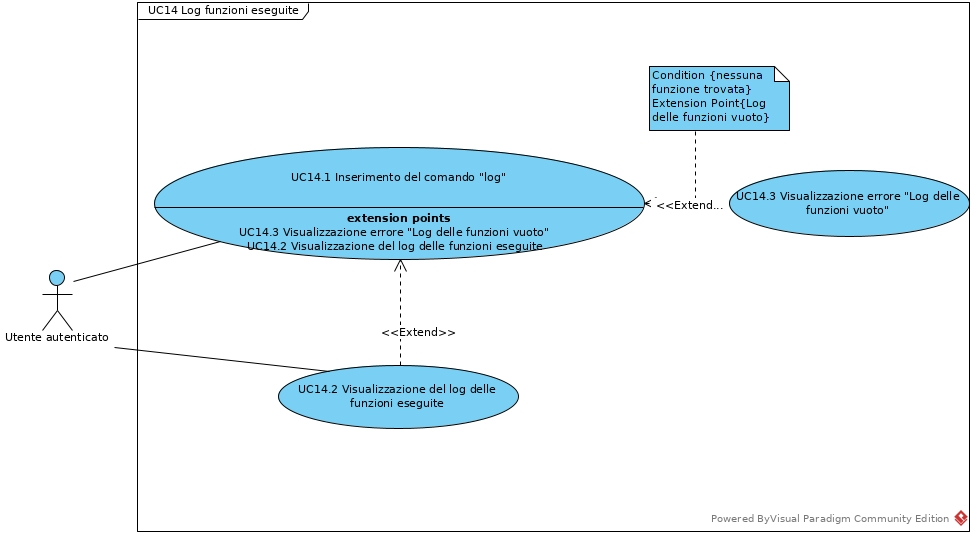
\includegraphics[width=\linewidth]{res/img/UC14.jpg}
	\caption{Diagramma UC14 - Elenco funzioni disponibili}
\end{figure}
\begin{itemize}
	\item \textbf{Attori primari:} Utente autenticato;
	\item \textbf{Descrizione:} l'utente visualizza la lista delle funzioni disponibili mediante il comando "list"; 
	\item \textbf{Pre-condizioni:} l'utente ha utilizzato il comando per la visualizzazione della lista delle funzioni rese disponibili dagli sviluppatori;
	\item \textbf{Post-condizioni:} il sistema visualizzerà sulla \textit{CLI\glo} l'elenco delle funzioni;
	\item \textbf{Scenario principale:} 
	\begin{enumerate}
		\item L'utente richiede l'elenco mediante comando "list";
		\item Il sistema visualizzerà su schermo la lista delle funzioni specificandone le principali informazioni.
%		\begin{itemize}
%			\item nome;
%			\item firma;
%			\item costo;
%			\item descrizione.
%		\end{itemize}
	\end{enumerate}
\end{itemize}